
\chapter{  Sprint 1 : Gestion des accès}

\section*{Introduction}
\addcontentsline{toc}{section}{Introduction}
Dans ce sprint, l'équipe s'est concentrée sur la mise en place des fonctionnalités de base, notamment l'authentification des utilisateurs, la déconnexion sécurisée, la gestion des utilisateurs et la définition des rôles. Ces éléments sont essentiels pour assurer la sécurité et la convivialité de l'application, ainsi que pour permettre une gestion efficace des utilisateurs et de leurs autorisations.

%________________________________________________________________________________________________________________

\section{Backlog du sprint 1}
Le backlog du sprint présente un ensemble des fonctionnalités extraites par l’équipe scrum à partir du backlog de produit et qui vont être réalisés pendant ce sprint. Les tâches à achever
pendant notre premier sprint sont présentées dans le tableau 3.1 suivant :

\begin{table}[H]
  \centering
  \renewcommand{\arraystretch}{1}
  \begin{tabular}{|c|c|p{7.5cm}|c|}
    \hline
    \textbf{ID}  & \textbf{Fonctionnalités} & \centering \textbf{User Story}                                                                                             & \textbf {Story points} \\
    \hline
    \textbf{US1} & Authentification         & En tant qu'admin, chauffeur, chef d'équipe et mécanicien je veux m'authentifier pour que j'accède à mon espace.            & 3                      \\
    \hline
    \textbf{US2} & Déconnexion              & En tant qu'admin, chauffeur, chef d'équipe et mécanicien je veux me déconnecter pour que je quitte l'application.          & 1                      \\
    \hline
    \textbf{US3} & Modification profil      & En tant qu'admin, chauffeur, chef d'équipe et mécanicien je veux modifier mon profil pour modifier photo et mots de passe. & 3                      \\
    \hline
    \textbf{US4} & Gestion des utilisateurs & En tant qu'admin je veux Gérer les utilisateurs pour que je puisse les ajouter,modifier et supprimer .                     & 5                      \\
    \hline
    \textbf{US5} & Gestion des rôles        & En tant qu'admin, je veux pouvoir gérer les rôles et les autorisations des utilisateurs.                                   & 2                      \\
    \hline
  \end{tabular}
  \caption{Backlog du sprint 1}

\end{table}

%__________________________________________________________________________________________________________________________________________________________________________________
\newpage
\section{Analyse et conception}
La section "Analyse et Conception" présente les méthodes de conception et la structure de notre application. Elle présente les diagrammes de cas d'utilisation, qui identifient les interactions des utilisateurs avec le système, les diagrammes de séquences système, qui illustrent l'ordre des opérations et la coordination entre les composants du système, et les diagrammes de classes participantes, qui dépeignent la structure objet et les relations entre les classes. Ces diagrammes sont essentiels pour comprendre le fonctionnement interne et l'architecture de l'application, afin de  répondre aux besoins des utilisateurs

%________________________________________________________________________________________________________________

\subsection{Diagramme de cas d’utilisation du sprint 1}

Ce diagramme illustre les différentes interactions que les utilisateurs peuvent avoir avec notre application. Il sert à identifier clairement les fonctionnalités accessibles par chaque type d'utilisateur et à définir les exigences système nécessaires pour ces interactions.

\begin{figure}[ht!]
  \centering
  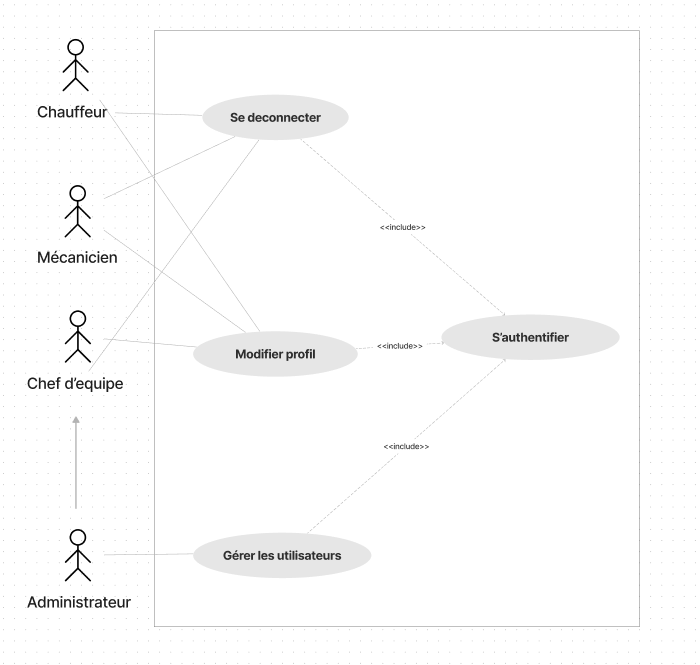
\includegraphics[width=1\textwidth,height=14cm]{chap3.images/usecase global sprint 1.png}
  \caption{Diagramme de cas d’utilisation global du sprint 1}

\end{figure}

%________________________________________________________________________________________________________________



\newpage
\subsection{Description textuelle du cas d’utilisation “S’authentifier”}

\begin{table}[H]
  \centering
  \renewcommand{\arraystretch}{1.2}
  \begin{tabular}{|p{4cm}|p{9cm}|}
    \hline
    \textbf{Cas d'utilisation}   & S'authentifier                                                                                                                   \\
    \hline
    \textbf{Acteur}              & Administrateur, Chef d’équipe, Chauffeur et Mécanicien                                                                           \\
    \hline
    \textbf{Pré-condition}       & L'utilisateur accède à l'interface d'authentification de l'application.                                                          \\
    \hline
    \textbf{Post-condition}      & L'utilisateur est authentifié et accède à son espace sécurisé dans l'application.                                                \\
    \hline
    \textbf{Scenario nominal}    & 1- L'utilisateur saisit son identifiant et son mot de passe.\newline

    2- L'utilisateur appuie sur le bouton de confirmation.\newline

    3- Le système vérifie les informations d'identification fournies par l'utilisateur. \newline

    4- L'utilisateur est redirigé vers son espace sécurisé dans l'application.                                                                                      \\


    \hline
    \textbf{Scénario alternatif} & A1 identifiants / mot de passe erroné :                                                                                 \newline

    l'enchainement A1 démarre au point 3 du scénario nominal. \newline

    4- un message d'erreur va etre afficher. \newline

    Le scénario nominal reprend au point 1.                                                                                                                         \\
    \hline
  \end{tabular}
  \caption{Description textuelle du cas d’utilisation “S’authentifier”}

\end{table}
%________________________________________________________________________________________________________________

\newpage
\subsection{Diagramme de séquence système du cas d’utilisation «S’authentifier»}
Un diagramme de séquences système est une représentation graphique qui illustre les interactions entre les acteurs ou les composants d'un système informatique pour accomplir une série d'actions ou de processus. Il met en évidence la chronologie des échanges de messages entre ces entités, fournissant ainsi une vue détaillée de la façon dont le système fonctionne pour atteindre ses objectifs.

\bigskip
\begin{figure}[ht!]
  \centering
  \includegraphics[width=1\textwidth,height=18cm]{chap3.images/Dss S’authentifier.png}
  \caption{Diagramme de séquence système du cas d’utilisation « S’authentifier » }

\end{figure}

%________________________________________________________________________________________________________________
\newpage

\subsection{Raffinement du cas d'utilisation « Gérer les utilisateurs »}

\begin{figure}[ht!]
  \centering
  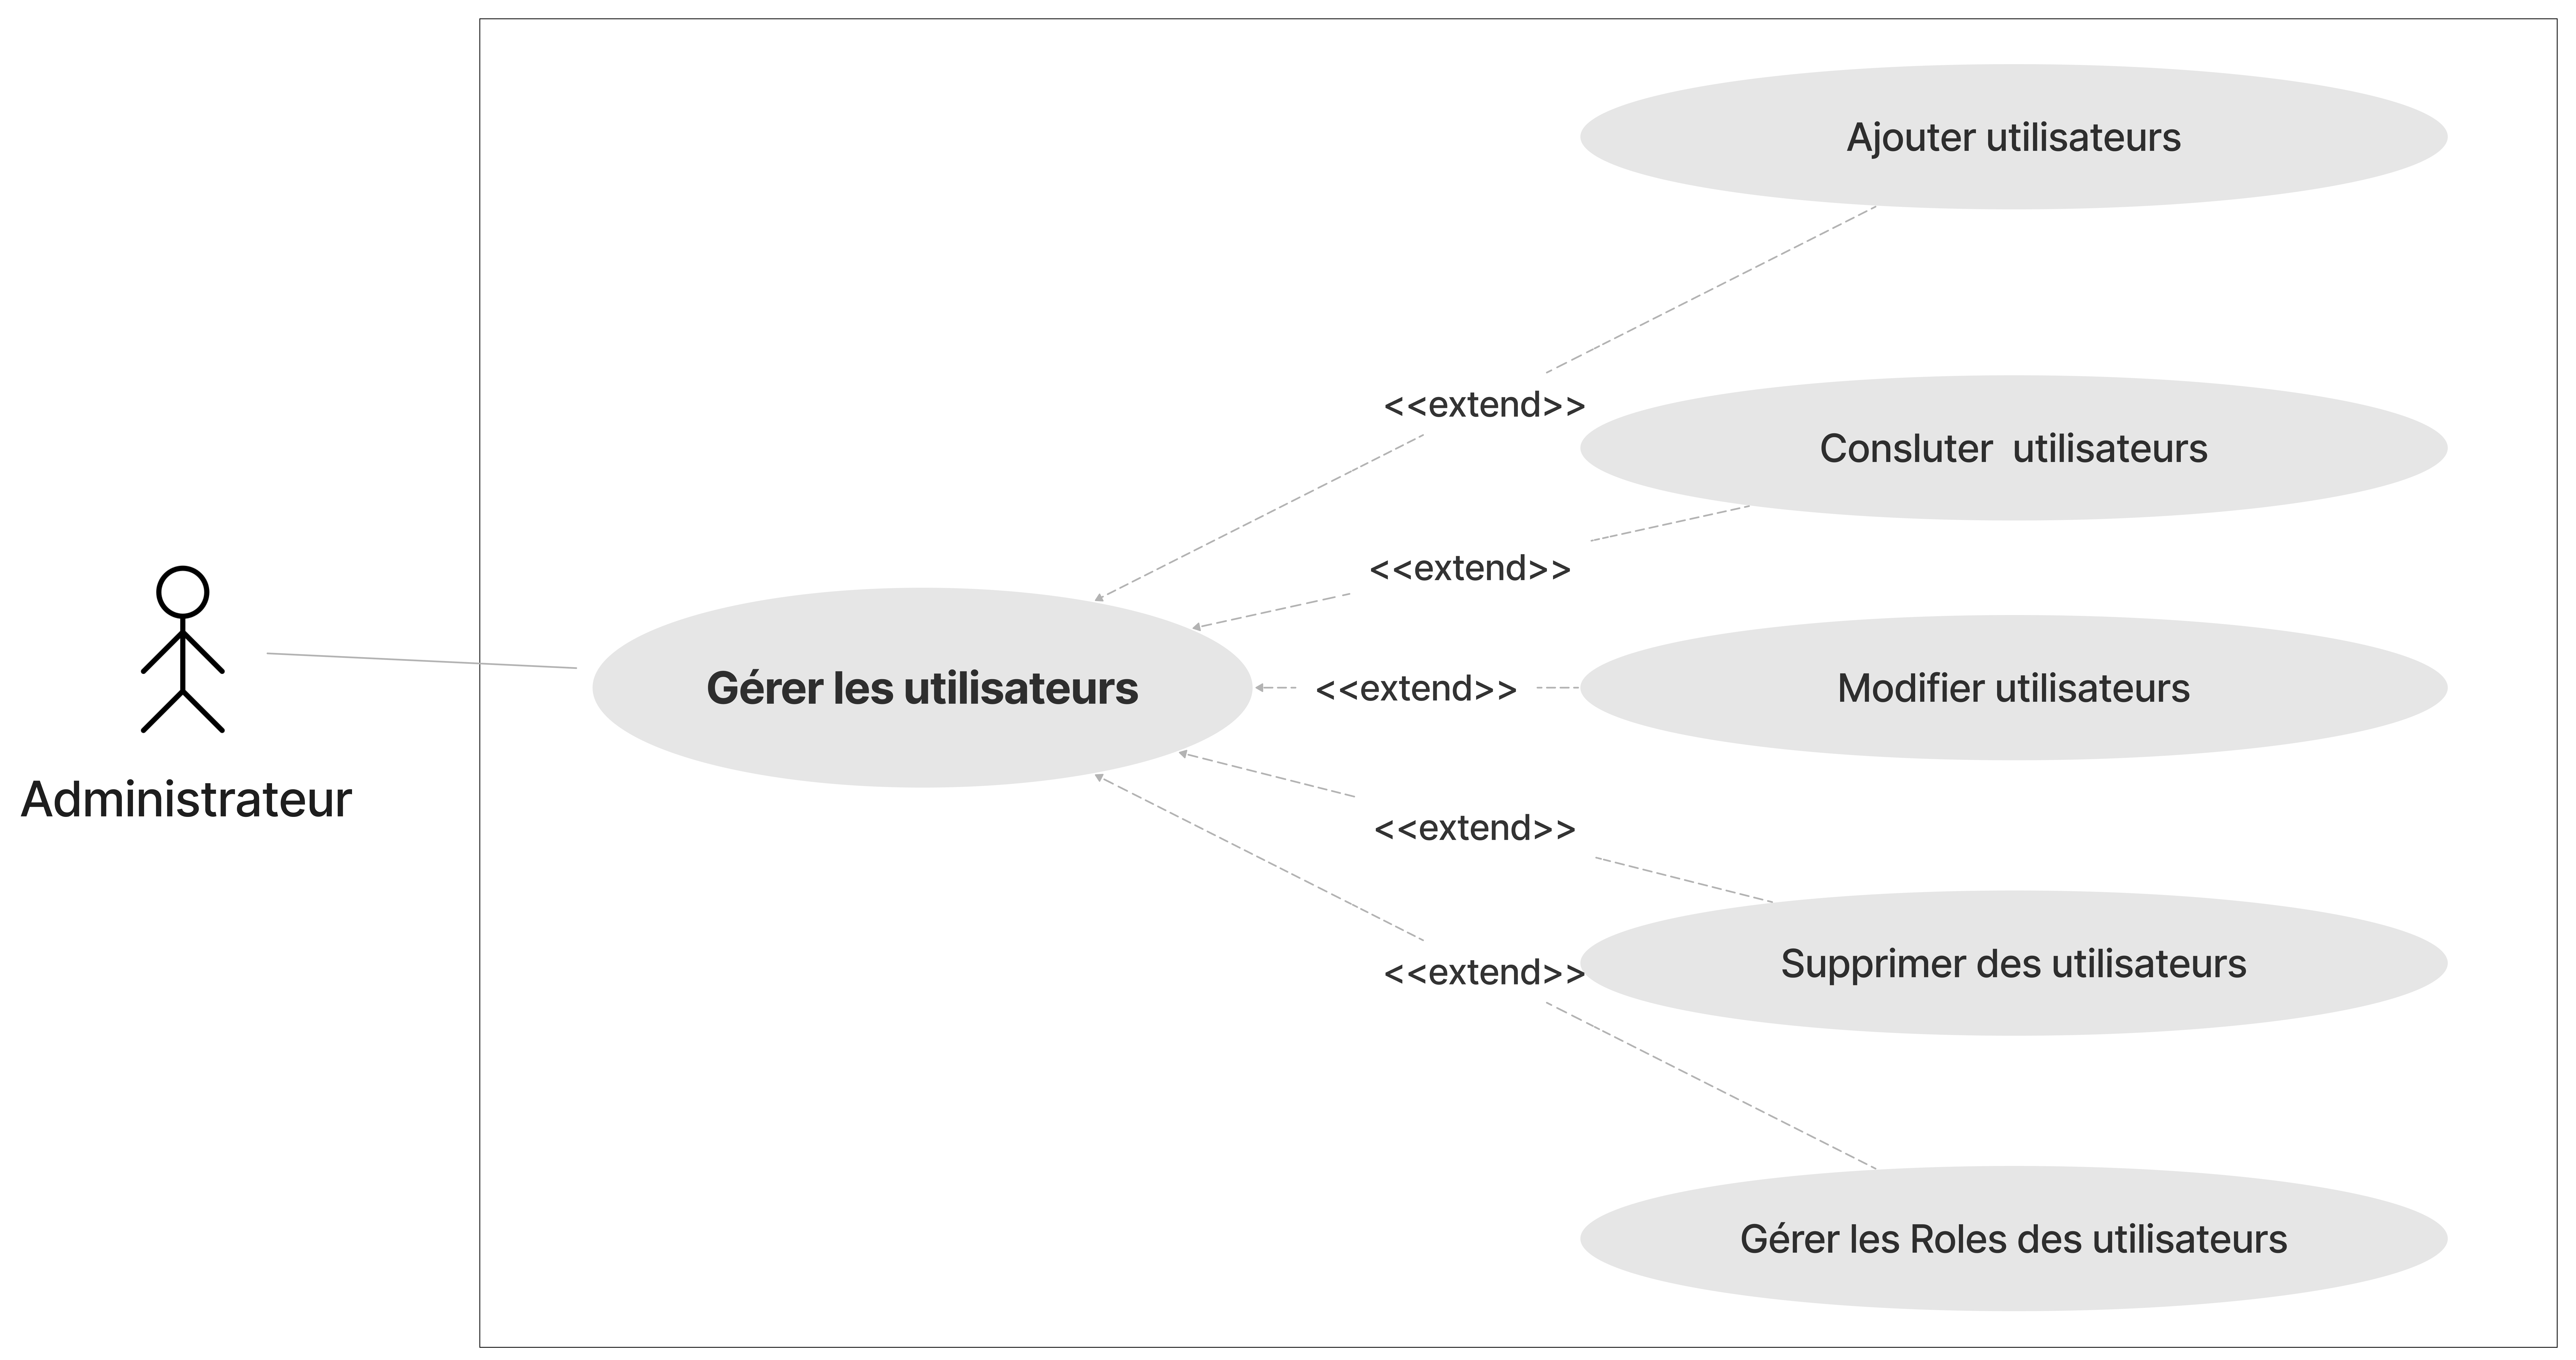
\includegraphics[width=1\textwidth,height=6cm]{chap3.images/gerer raf sprint 1.png}
  \caption{Analyse de cas d’utilisation « Gérer les utilisateurs »}

\end{figure}

%________________________________________________________________________________________________________________


\subsection{Description textuelle du cas d’utilisation “Ajouter utilisateur”}
\begin{table}[H]
  \centering
  \renewcommand{\arraystretch}{1.1}
  \begin{tabular}{|p{4cm}|p{9cm}|}
    \hline
    \textbf{Cas d'utilisation}   & Ajouter Utilisateur                                                                                           \\
    \hline
    \textbf{Acteur}              & Administrateur                                                                                                \\
    \hline
    \textbf{Pré-condition}       & L'administrateur est authentifié dans le système .                                                            \\
    \hline
    \textbf{Post-condition}      & Le nouvel utilisateur est ajouté avec succès dans le système et peut accéder aux fonctionnalités appropriées. \\
    \hline
    \textbf{Scenario nominal}    & 1- L'administrateur accède à l'interface de gestion des utilisateurs.\newline

    2- L'administrateur ajoute un nouvel utilisateur en saisissant ses informations dans un formulaire dédié.\newline

    3- Le système vérifie les informations saisies.\newline
    
    4- Le nouvel utilisateur est ajouté à la base de données.\newline

    5- Le système envoie un e-mail au nouvel utilisateur contenant ses informations de connexion pour accéder au système.                        \\
    \hline
    \textbf{Scénario alternatif} & A1 Erreur de saisie des informations : \newline

    l'echainement A1 démarre au point 3 du scenario nominal.                                                                                     \\
  \end{tabular}

\end{table}


\begin{table}[H]
  \centering
  \renewcommand{\arraystretch}{1.1}
  \begin{tabular}{|p{4cm}|p{9cm}|}

     & 4- Le système affiche un message pour verifier les informations saisies.\newline

    Le scénario nominal reprend au point 2.                                             \\

    \hline
  \end{tabular}
  \caption{Description textuelle du cas d’utilisation “Ajouter utilisateur”}



\end{table}

%________________________________________________________________________________________________________________

\subsection{Diagramme de séquence système du cas d’utilisation «Ajouter utilisateur»}

\begin{figure}[ht!]
  \centering
  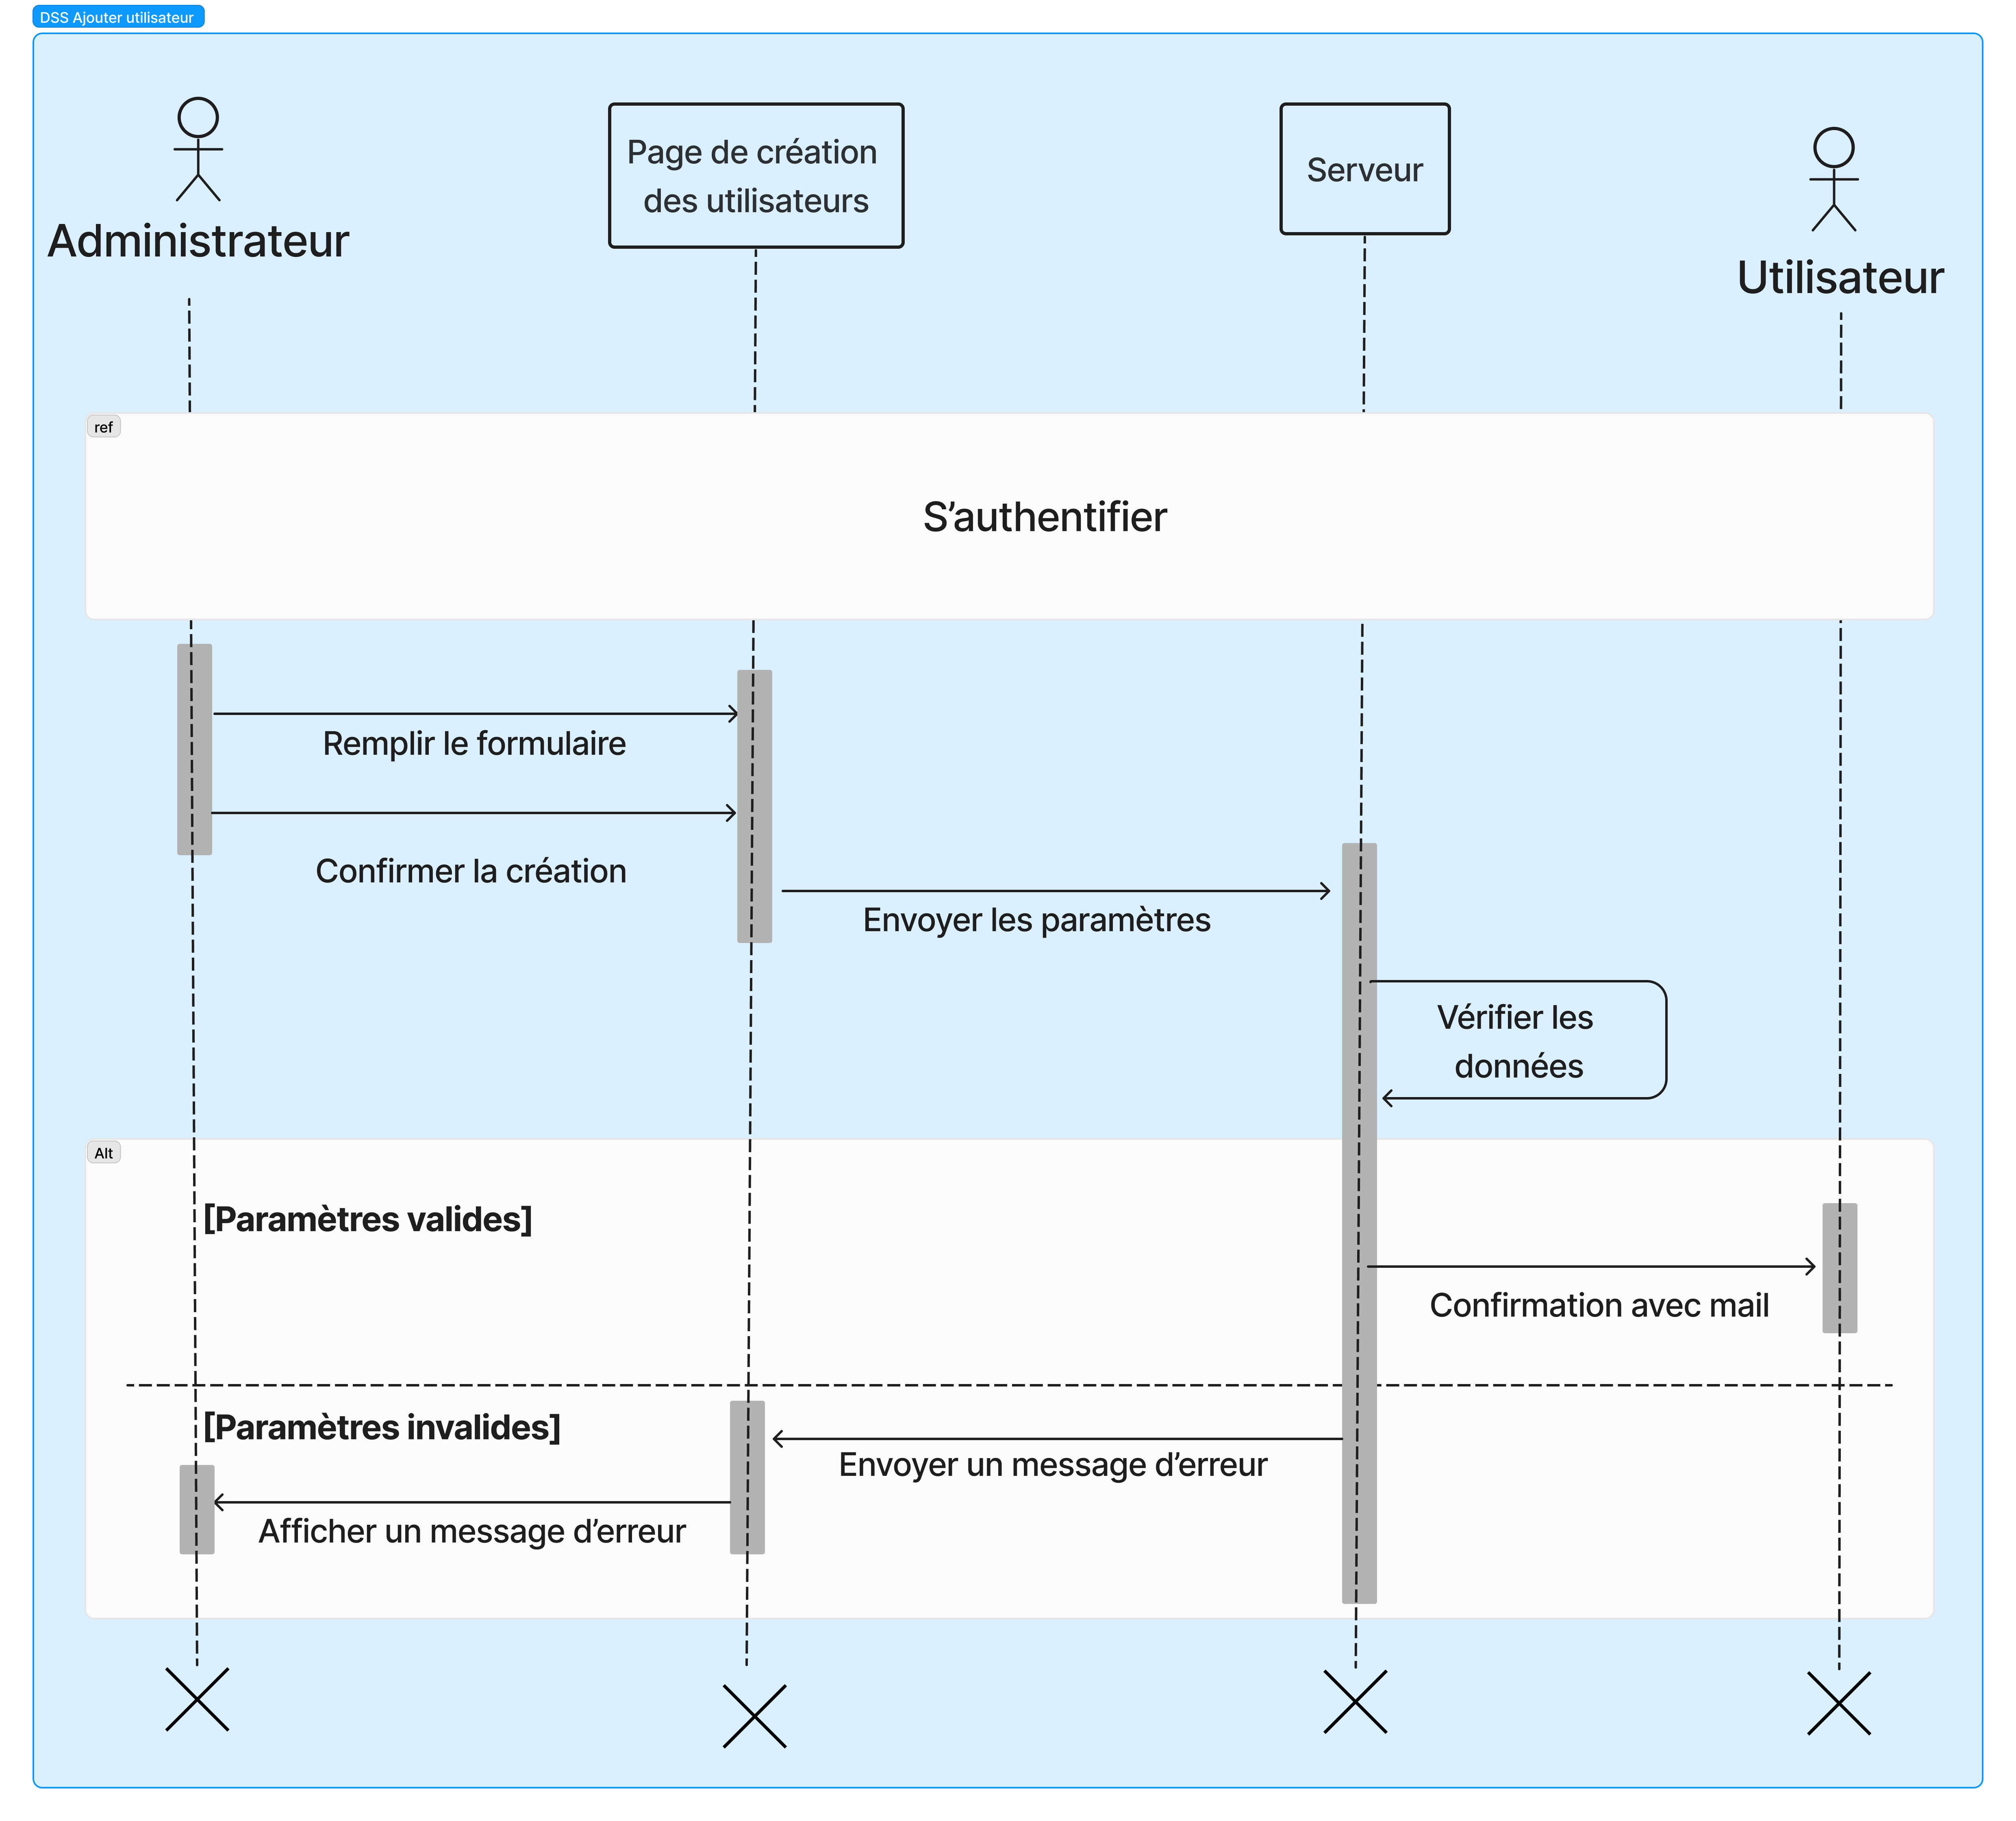
\includegraphics[width=1\textwidth,height=17.5cm]{chap3.images/DSS ajouter utilisateur.png}
  \caption{ Diagramme de séquence système du cas d’utilisation «Ajouter utilisateur» }
\end{figure}
%________________________________________________________________________________________________________________
%________________________________________________________________________________________________________________
\newpage
\section{Diagramme de classes du sprint 1}

\begin{figure}[ht!]

  \centering
  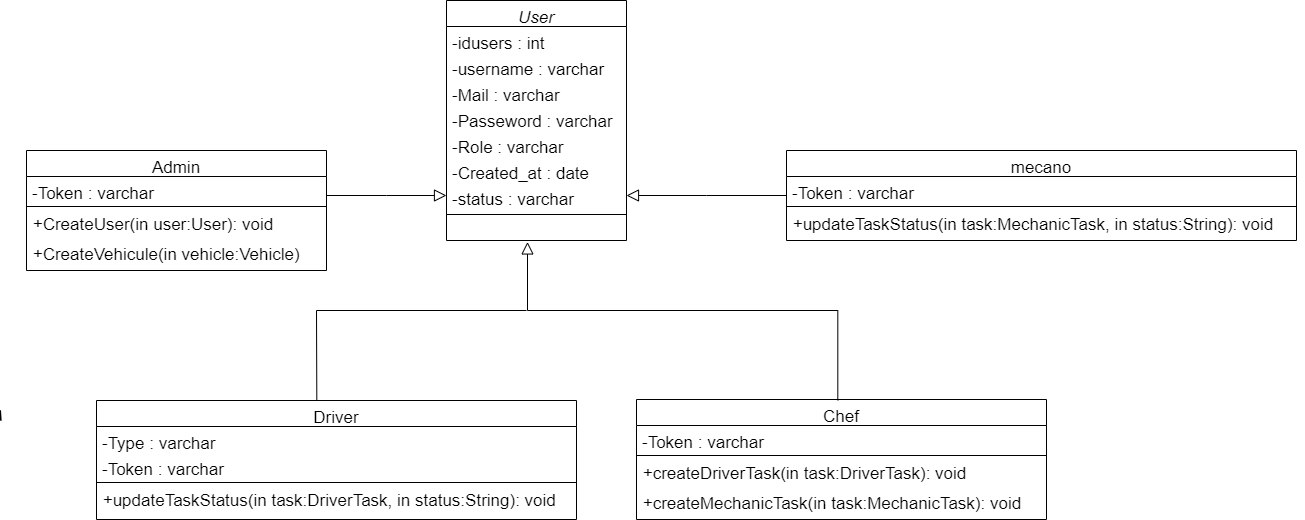
\includegraphics[width=1\textwidth,height=9cm]{chap3.images/class sprint 1.png}
  \caption{Diagramme de classes du sprint 1}

\end{figure}

%________________________________________________________________________________________________________________
\newpage
\section{ Réalisation}

Dans cette section, nous mettons en lumière les interfaces  de l'application que nous avons développée. À travers des captures d'écran détaillées, nous illustrons les fonctionnalités clés mises à disposition des utilisateurs, démontrant ainsi l'application pratique des concepts et des designs discutés dans les sections précédentes.



\subsection{Authentification}
Cette interface permet au utilisateurs de se connecter à l'application . L'utilisateur est accueilli par un formulaire de connexion simple, comprenant des champs pour saisir son identifiant et son mot de passe. Une fois les informations d'identification saisies, l'utilisateur peut appuyer sur le bouton  'confirmer' pour accéder à son espace sécurisé, si les informations d'identification saisies sont incorrectes, le système affiche un message d'erreur. \\


\begin{figure}[ht!]
  \centering
  \includegraphics[width=0.9\textwidth,height=6.5cm]{chap3.images/Authentification web.png}
  \caption{Interface d'authentification Web }

\end{figure}
\begin{figure}[ht!]
  \centering
  \includegraphics[width=0.9\textwidth,height=6.5cm]{chap3.images/authentification échoué.png}
  \caption{Echec de connexion }

\end{figure}

%________________________________________________________________________________________________________________

\newpage

\begin{figure}[htbp]
  \centering
  \begin{minipage}{0.45\textwidth}
    \centering
    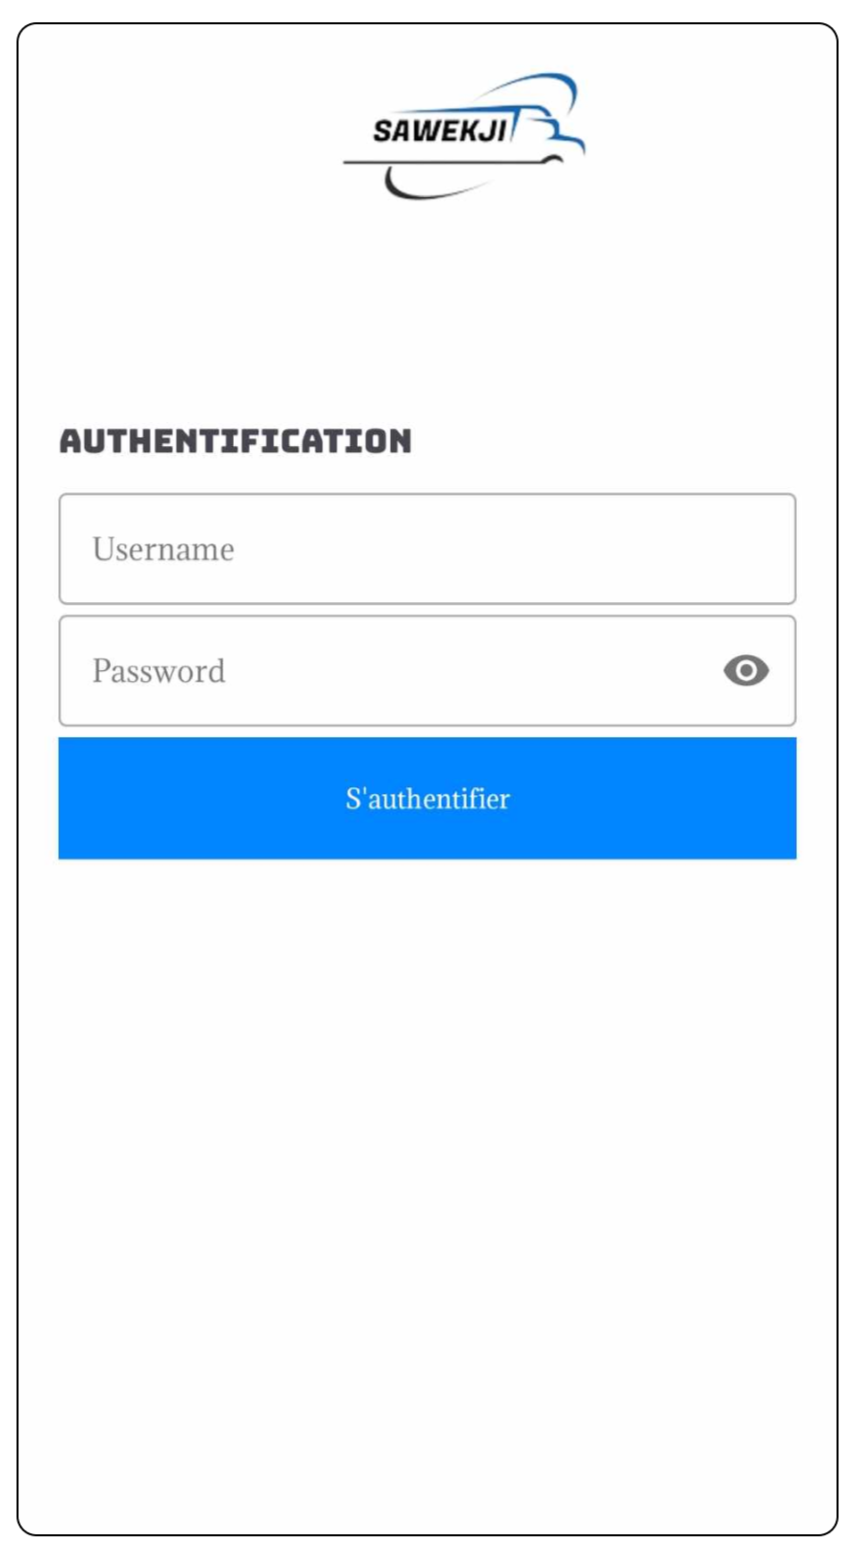
\includegraphics[width=0.7\textwidth,height=8cm]{chap3.images/authentfication mob.png}
    \caption{\centering{Interface d'authentification Mobile}}

  \end{minipage}
  \hfill
  \begin{minipage}{0.45\textwidth}
    \centering
    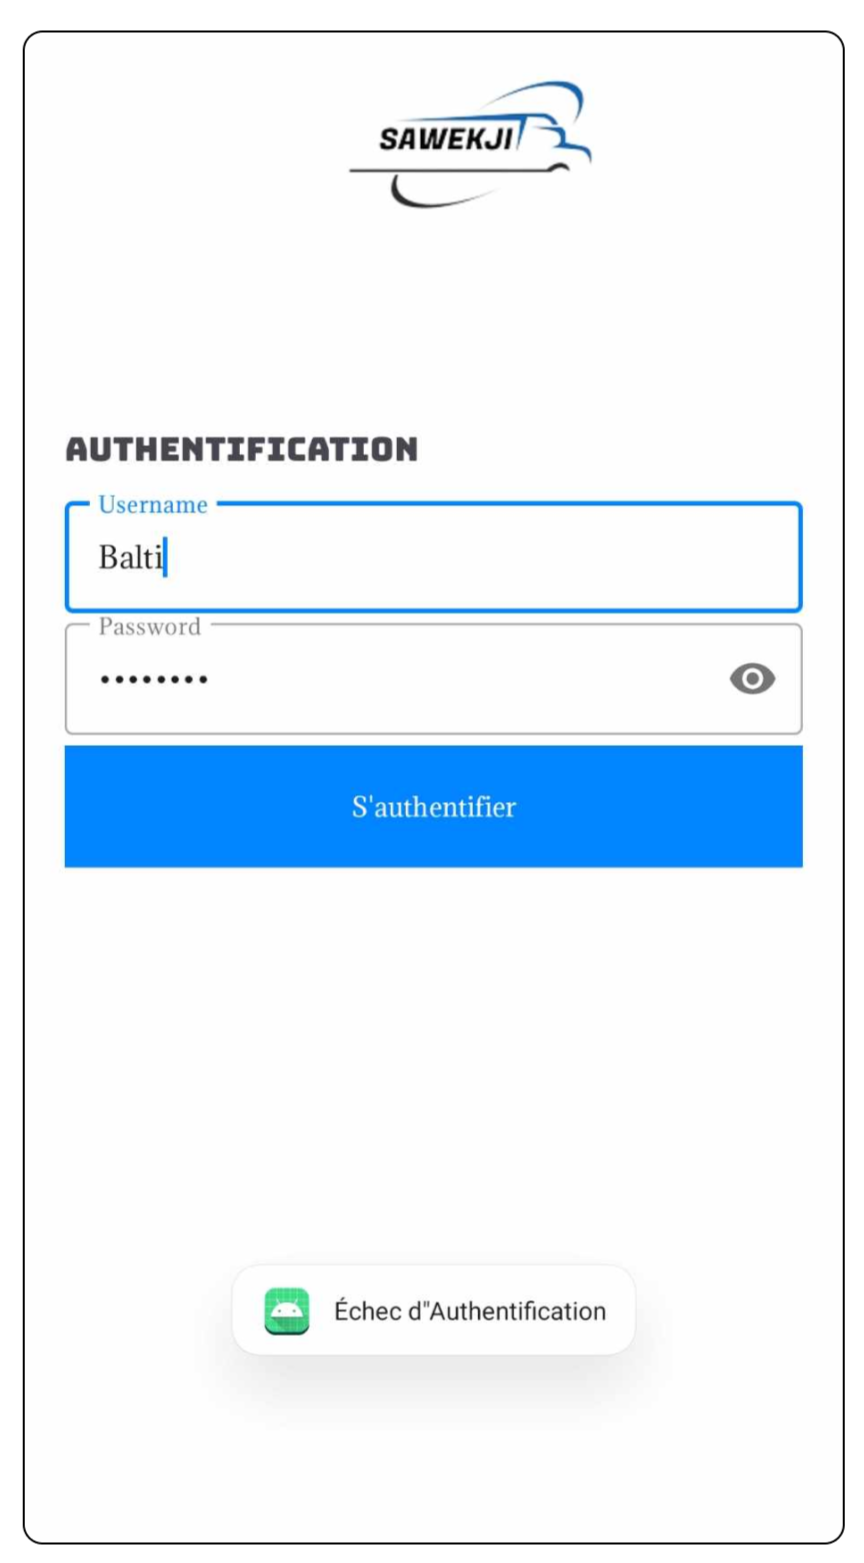
\includegraphics[width=0.7\textwidth,height=8cm]{chap3.images/echec authentification mob.png}
    \caption{Echec de connexion }

  \end{minipage}
\end{figure}


\vspace{1.2cm}
%________________________________________________________________________________________________________________

\subsection{ Profil}

Permet à l'administrateur, chef d'équipe, chauffeur et mécanicien de changer leur photo de profil et leur mot de passe.

\begin{figure}[h!]
  \centering
  \begin{minipage}[t]{0.59\textwidth}
    \centering
    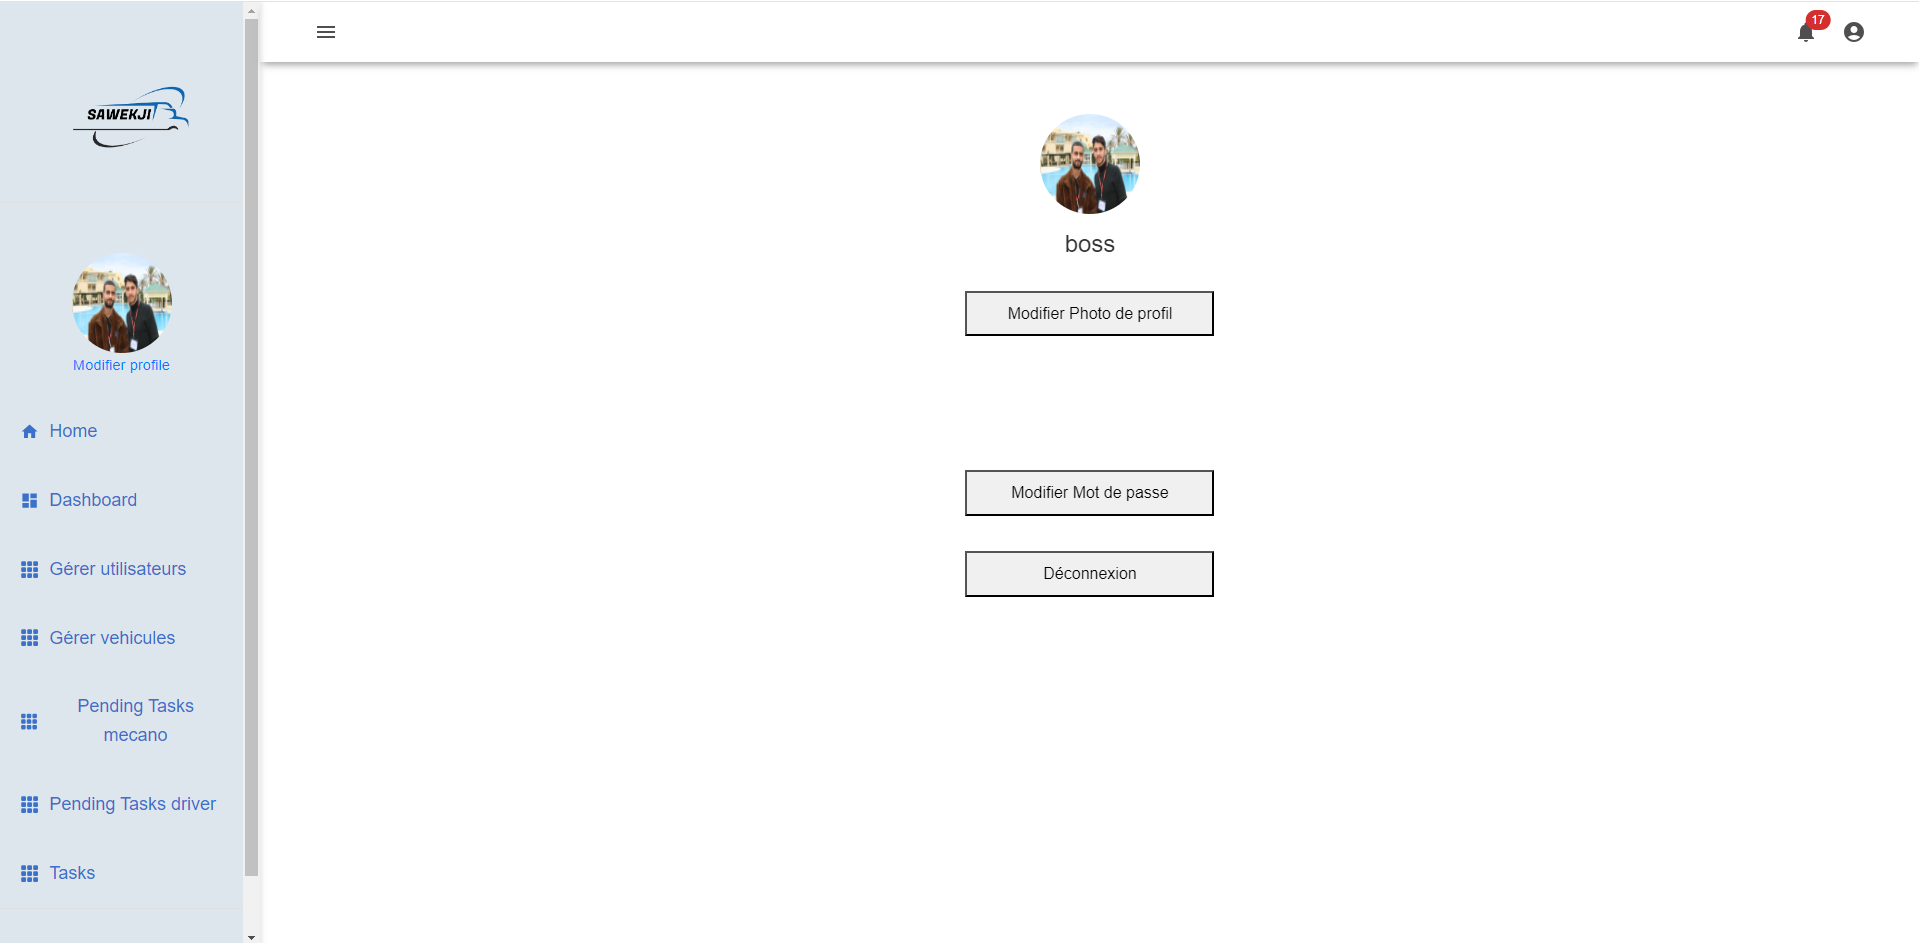
\includegraphics[width=1\textwidth, height=6cm]{chap3.images/modifier profil (web).png}
    \caption{Interface de profil  - Web}
  \end{minipage}
  \hfill
  \begin{minipage}[t]{0.39\textwidth}
    \centering
    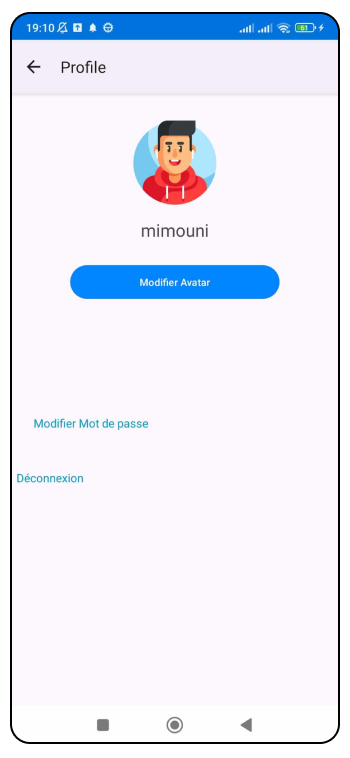
\includegraphics[width=0.7\textwidth, height=7.5cm]{chap3.images/modifier profil mobile.png}
    \caption{\centering{Interface de profil - Mobile}}
  \end{minipage}
\end{figure}

%%%%%%%%%%%%%%%%%%%%%%%%%%%%%%%%%%%%%%%%%
\newpage
\subsection{Gestion des utilisateurs}
Lorsque l'administrateur accède à cette interface, il est présenté avec un tableau répertoriant tous les utilisateurs de l'application. Chaque ligne du tableau représente un utilisateur et affiche des informations telles que le nom, l'adresse e-mail et le rôle. L'administrateur a la possibilité de supprimer un utilisateur en cliquant sur l'icône de suppression correspondante dans la ligne de l'utilisateur. De plus, en cliquant sur l'icône de modification, l'administrateur peut mettre à jour les informations d'un utilisateur existant.
\bigskip

\begin{figure}[ht!]
  \centering
  \includegraphics[width=0.9\textwidth]{chap3.images/Gérer user.png}
  \caption{Interface de gestion des utilisateurs}

\end{figure}

%%%%%%%%%%%%%%%%%%%%%%%%%%%%%%%%%%%%%%%%%

\subsection{Création d'un nouvel utilisateur}
Lorsque l'administrateur clique sur le bouton "Ajouter Utilisateur" dans l'interface précédente, un formulaire d'ajout d'utilisateur s'affiche à l'écran. Ce formulaire permet à l'administrateur de saisir les informations nécessaires pour créer un nouvel utilisateur, telles que le nom, l'adresse e-mail et le mot de passe initial. L'administrateur peut également sélectionner le rôle de l'utilisateur parmi les options disponibles. Une fois que toutes les informations requises sont fournies, l'administrateur peut soumettre le formulaire pour créer un nouvel utilisateur dans le système.\\

\newpage
\begin{figure}[ht!]
  \centering
  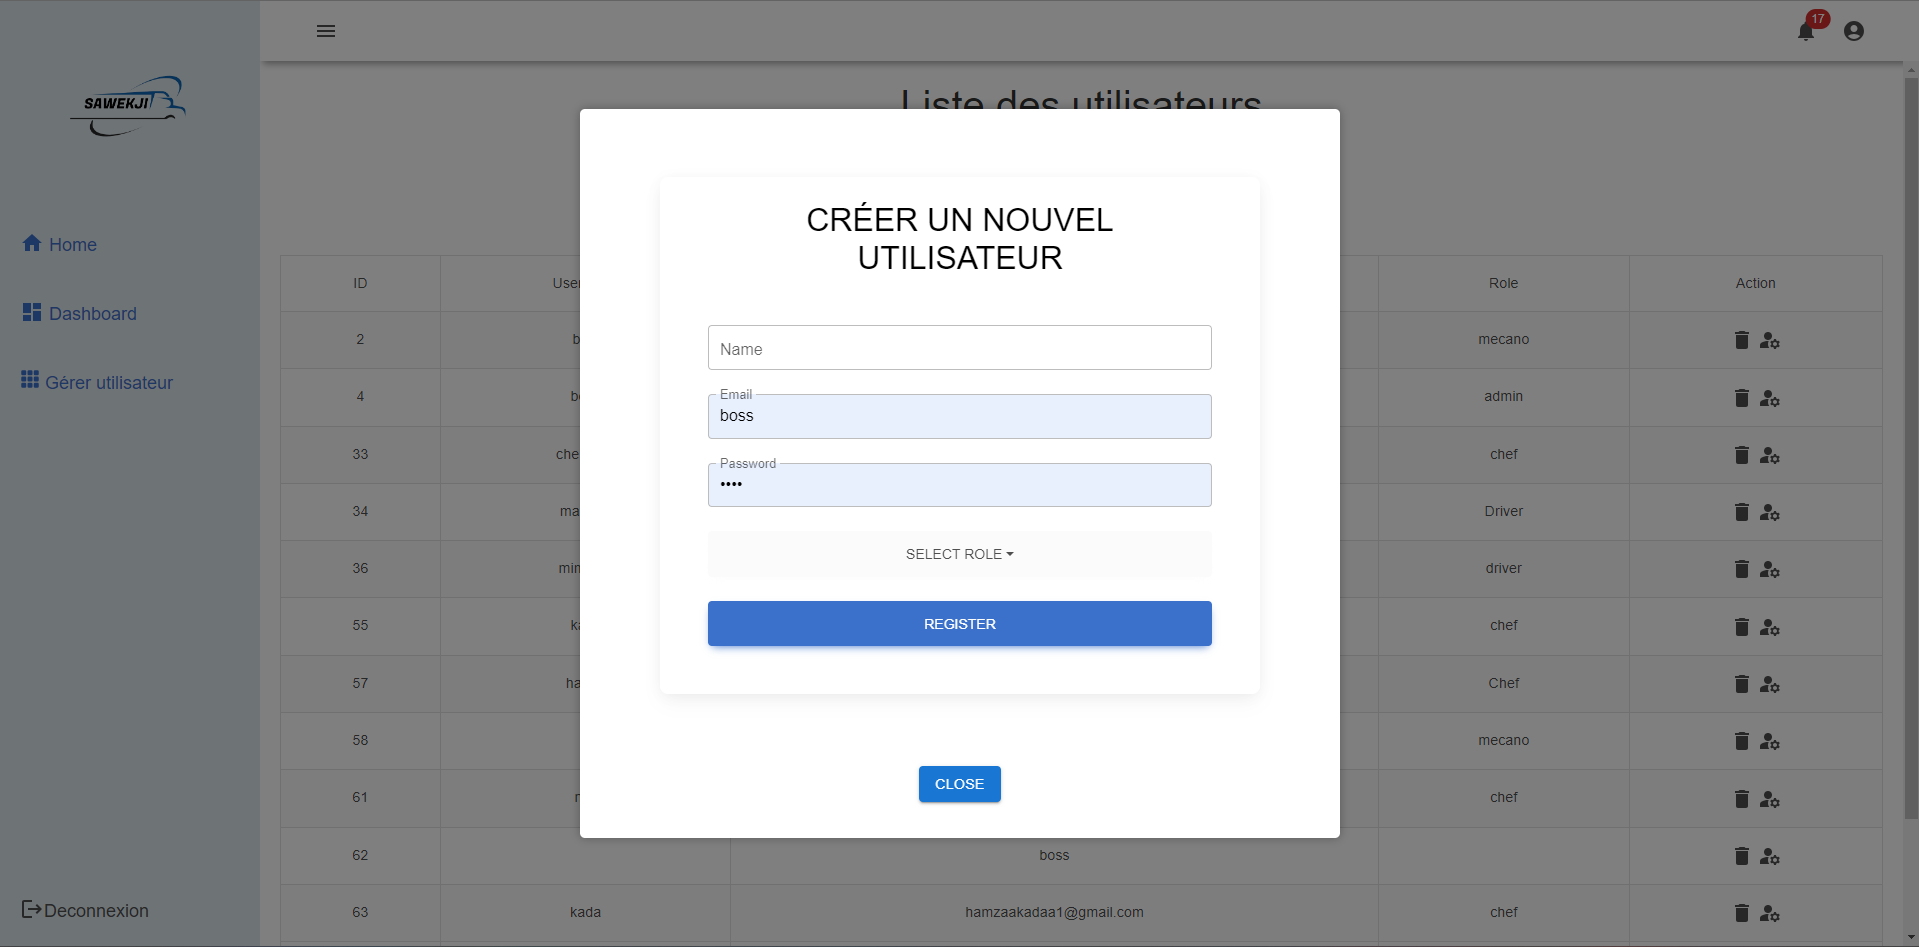
\includegraphics[width=0.9\textwidth,height=7cm]{chap3.images/creer user.png}
  \caption{Interface de création d'un nouvel utilisateur}

\end{figure}
%________________________________________________________________________________________________________________
\section{Rétrospective}
Dans cette section de rétrospective, nous examinerons de près les performances de notre équipe pendant le Sprint 1 en utilisant deux outils essentiels de la méthodologie Scrum : le burndown chart et le task board. Ces outils nous permettent de visualiser et d'évaluer notre progression tout au long du sprint.

\subsection{Burdown Chart}
Le burndown chart est un outil essentiel utilisé dans la gestion de projet agile pour suivre la progression des tâches. Il illustre graphiquement la quantité de travail restant à accomplir par l'équipe au cours du sprint. Dans notre cas, nous avons planifié un sprint de 3 semaines, avec une moyenne de 5 heures de travail par jour.

\begin{figure}[ht!]
  \centering
  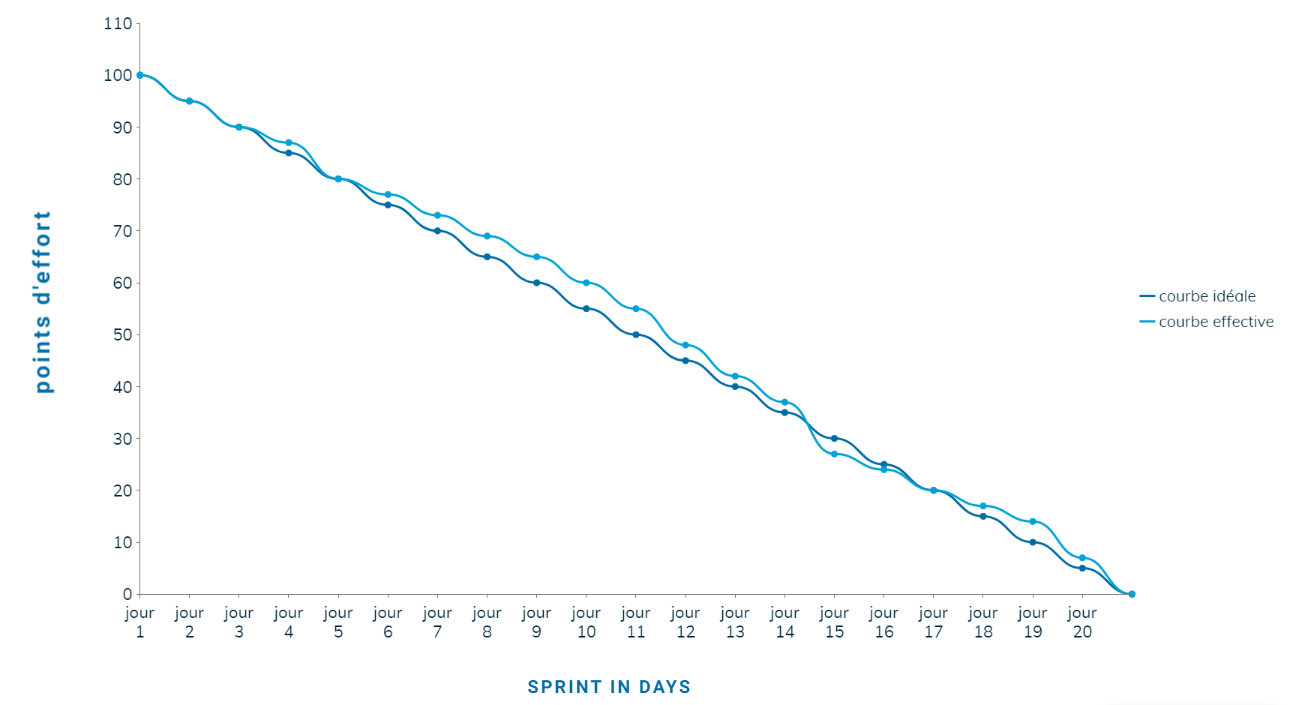
\includegraphics[width=1\textwidth, height=6.5cm]{chap3.images/burndown chart sprint 1.png}
  \caption{ Burdown Chart du Sprint 1}

\end{figure}
%%%%%%%%%%%%%%%%%%%%%%%%%%%%%%%%%%%%%%%%%

\newpage
\subsection{Task Bord}

La figure 3.14 présente le "Task Bord" correspondant au 6ème jour du sprint 1.

\begin{figure}[ht!]
  \centering
  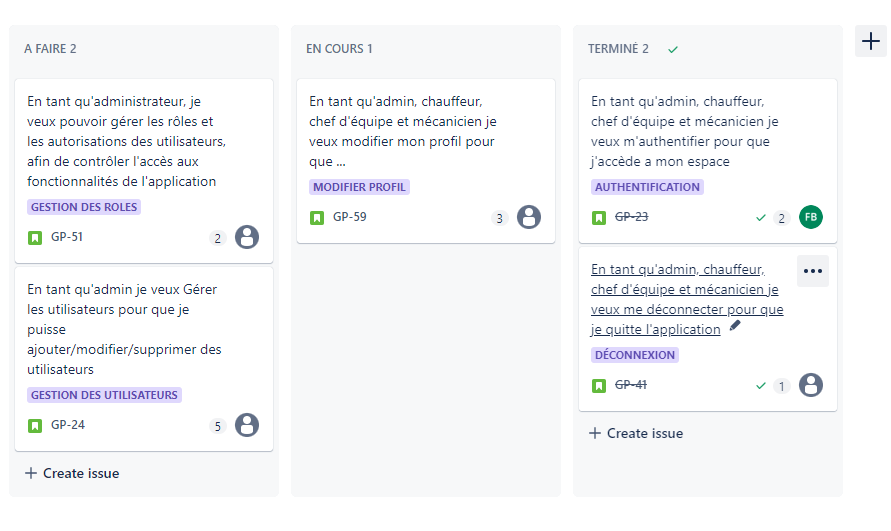
\includegraphics[width=0.9\textwidth, height=8cm]{chap3.images/task board sprint 1.png}
  \caption{ Task board du Sprint 1 }

\end{figure}
%_______________________________________________________________________________________________
\section{Tests unitaires}
Dans cette section, nous utiliserons l'outil Postman pour effectuer des tests unitaires sur notre application. Les tests unitaires consistent à vérifier le bon fonctionnement de chaque unité de code de manière isolée. Nous définirons des scénarios de test, configurerons des requêtes HTTP dans Postman, et écrirons des scripts pour valider les résultats renvoyés par chaque unité de code. Ces tests nous permettront de détecter les erreurs dès le stade de développement .\\\\
%_______________________________________________________________________________________________
\bigskip
\textbf{Test unitaires du cas d’utilisation « S'authentifier » :}\\
Nous présentons ci-dessous le code source et le résultat de deux cas de test :

1. Toutes les données sont valides.\newline
2. Mots de passe incorrecte .

\begin{figure}[ht!]
  \centering
  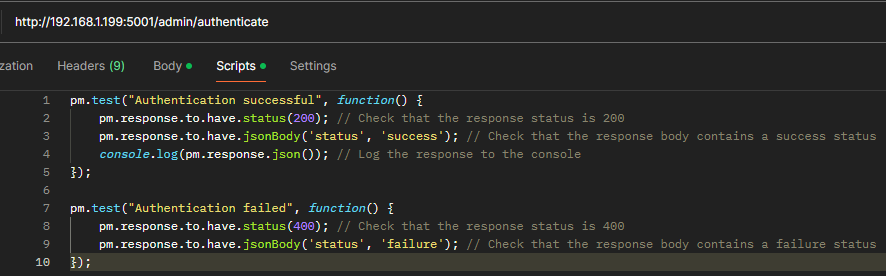
\includegraphics[width=0.7\textwidth, height=3.5cm]{chap3.images/code source test.png}
  \caption{ Code souce du test unitaire du cas d’utilisation «S’authentifier » }

\end{figure}

\newpage
\begin{figure}[ht!]
  \centering
  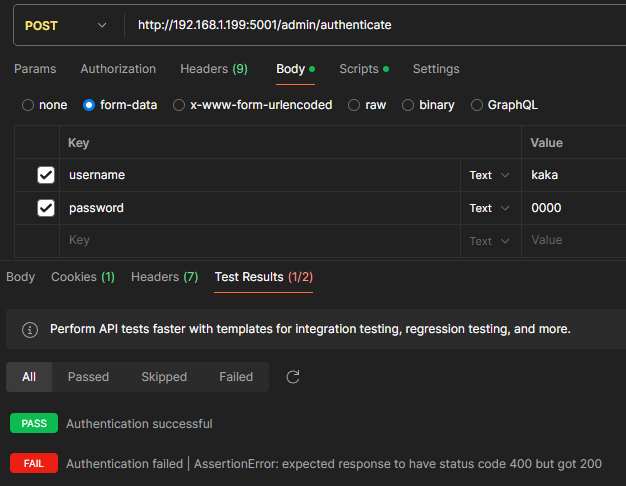
\includegraphics[width=0.7\textwidth, height=6.5cm]{chap3.images/cas1.png}
  \caption{ Resultat du premier test }

\end{figure}

\begin{figure}[ht!]
  \centering
  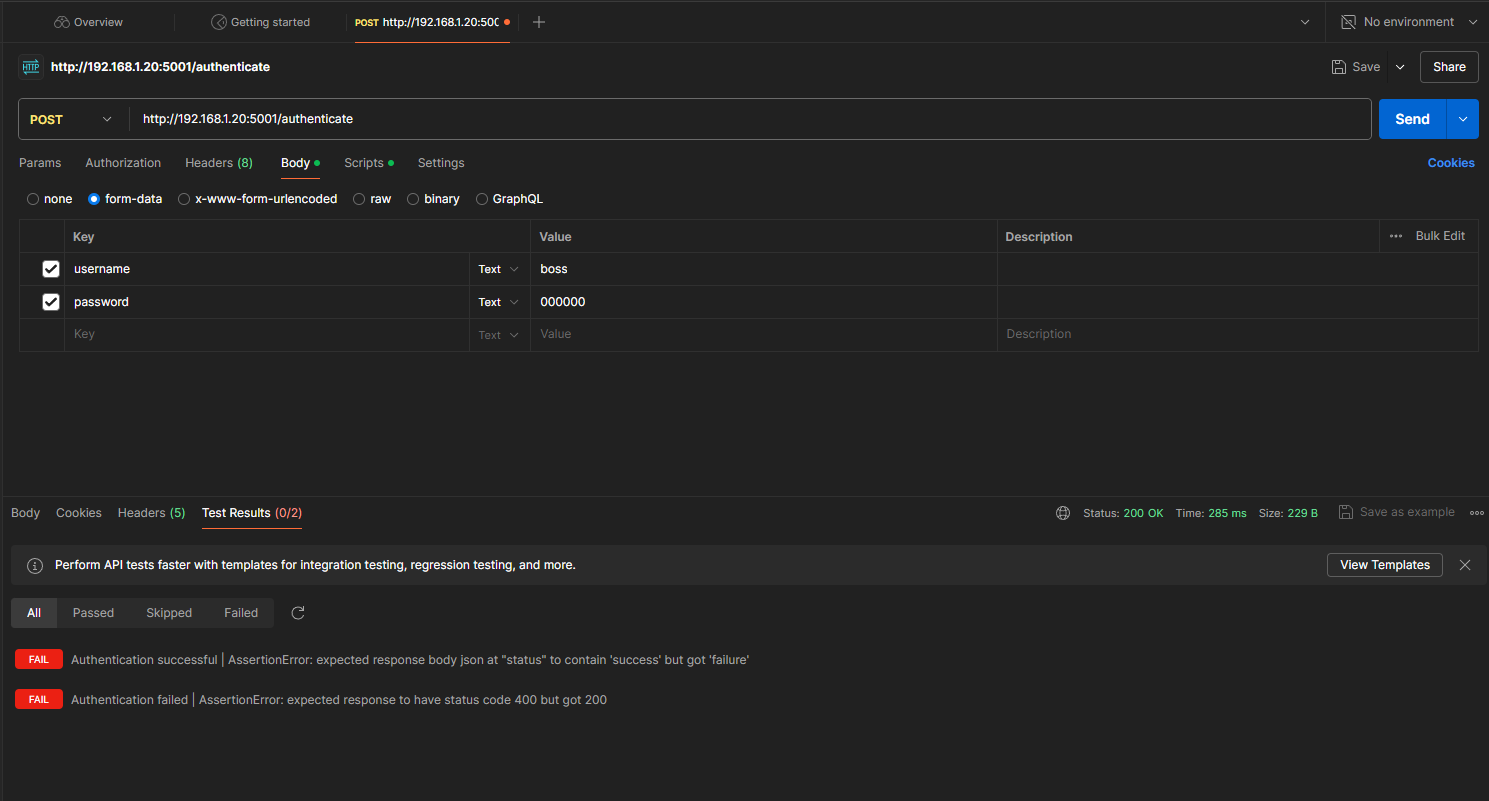
\includegraphics[width=0.7\textwidth, height=6.5cm]{chap3.images/cas2.png}
  \caption{ Resultat du deuxieme test }

\end{figure}
%_______________________________________________________________________________________________

\section*{Conclusion}
\addcontentsline{toc}{section}{Conclusion}
\bigskip
\begin{sloppypar}
  Dans ce chapitre, nous avons examiné en détail le premier Sprint, en décrivant le contenu du Sprint Backlog, le diagramme de cas d'utilisation et les séquences système des cas d'utilisation principaux. Nous avons également illustré quelques fonctionnalités de l'application à travers un scénario, et présenté d'autres outils de Scrum comme le Task Board et le burndown Chart. Dans le prochain chapitre, nous continuerons à explorer les fonctionnalités du deuxième Sprint.
\end{sloppypar}
